% !TEX TS-program = xelatex


\documentclass[a4paper,14pt]{extarticle}

% Include settings from setting.tex
\input{setting.tex}

\geometry{a4paper, margin=1in}
\graphicspath{{img/}}

\newcommand{\assignNum}{2} %change the number of the assignment here
\author{مرتضی ملکی‌نژاد شوشتری} %change your name here
\newcommand{\SNum}{810104256} %change your SID here
\date{\today}
\title{تمرین \assignNum}

\begin{document}
\pagenumbering{gobble}
\maketitle
\newpage
\tableofcontents

\newpage
\listoffigures

\newpage
\listoftables

\newpage
\pagenumbering{arabic}

\section{چکیده}
این تمرین برای تسلط روی 
\lr{Parzen}
، 
\lr{KNN}
،
\lr{Hypothesis Testing}
و توزیع 
$\chi^2$
و توزیع‌های مشتق از آن و استفاده‌های آن (مثلا توزیع واریانس) ارائه شده است.

\newpage
\setcounterref{section}{0}
\lr{\section{Parzen Window}}
\subsection{}
فرمول پارزن برابر است با:
\begin{latin}
	$
	\hat{P}(X) = \cfrac{1}{N} \sum\limits_{i=1}^{N} \cfrac{1}{h^d} \phi(\cfrac{x - x_i}{h})
	$
\end{latin}
که در این‌جا \lr{d} برابر یک است زیرا فقط یک بعد داریم.
چون هدف بدست آوردن میانگین  
$\hat{P}(X)$
می‌باشد، باید امید را به شیوه‌ای حساب کرد که در آن داده متغیر تصادفی باشد. (که در فرمول نهایی \lr{x} موجود باشد.) چون داده‌ها نیز از توزیع جامعه هستند، می‌توان احتمال را جایگذاری کرد. همچنین چون در فرمول \lr{parzen} داریم میانگین \lr{n} متغیر تصادفی را حساب می‌کنیم و می‌دانیم که امید یک متغیر \lr{iid} با امید میانگین همه برابر است می‌توان صرفا برای یک متغیر تصادفی حساب کرد. پس داریم:

\begin{latin}
	$
	E(\hat{P}(Y)) = \bigintss\limits_{0}^a  \cfrac{1}{h^d}\  \phi(\cfrac{x - y}{h}) \cfrac{1}{a}\  d_y
	= \cfrac{1}{ha} \bigintss\limits_{0}^a \phi (\cfrac{x - y}{h})  d_y
	$
\end{latin}
اگر \lr{x} از \lr{y} کمتر باشد مقدار $\phi$ صفر می‌شود. پس اگر \lr{x} از صفر کمتر باشد، مقدار داخل انتگرال همواره صفر است و خروجی صفر می‌شود. 

اگر \lr{x} بین صفر و \lr{a} باشد داریم:
\begin{latin}
	$
	E(\hat{P}(Y) | 0 < x \leq a) = \cfrac{1}{ha} \bigintss\limits_0^x \phi (\cfrac{x - y}{h})  d_y 
	=  \cfrac{1}{ha} \bigintss\limits_0^x e^{\cfrac{y - x}{h}} \\
	= \cfrac{1}{ha} [he^{\cfrac{y - x}{h}}]_0^x = \cfrac{1}{a} (1 - e^{\cfrac{-x}{h}})
	$
\end{latin}
اگر 
\lr{x}
از 
\lr{a}
بزرگ‌تر باشد داریم:
\begin{latin}
	$
	E(\hat{P}(Y) | 0 < x \leq a) = \cfrac{1}{ha} \bigintss\limits_0^a \phi (\cfrac{x - y}{h})  d_y 
	= \cfrac{1}{ha} \bigintss\limits_0^a e^{\cfrac{y - x}{h}} \\
	= \cfrac{1}{ha} [he^{\cfrac{y - x}{h}}]_0^a = \cfrac{1}{a} (e^{\cfrac{a-x}{h}} - e^{\cfrac{-x}{h}})
	= \cfrac{1}{a} (e^{\cfrac{a}{h} - 1}){e^{\cfrac{-x}{h}}}
	$
\end{latin}
\subsection{}
{
\centering
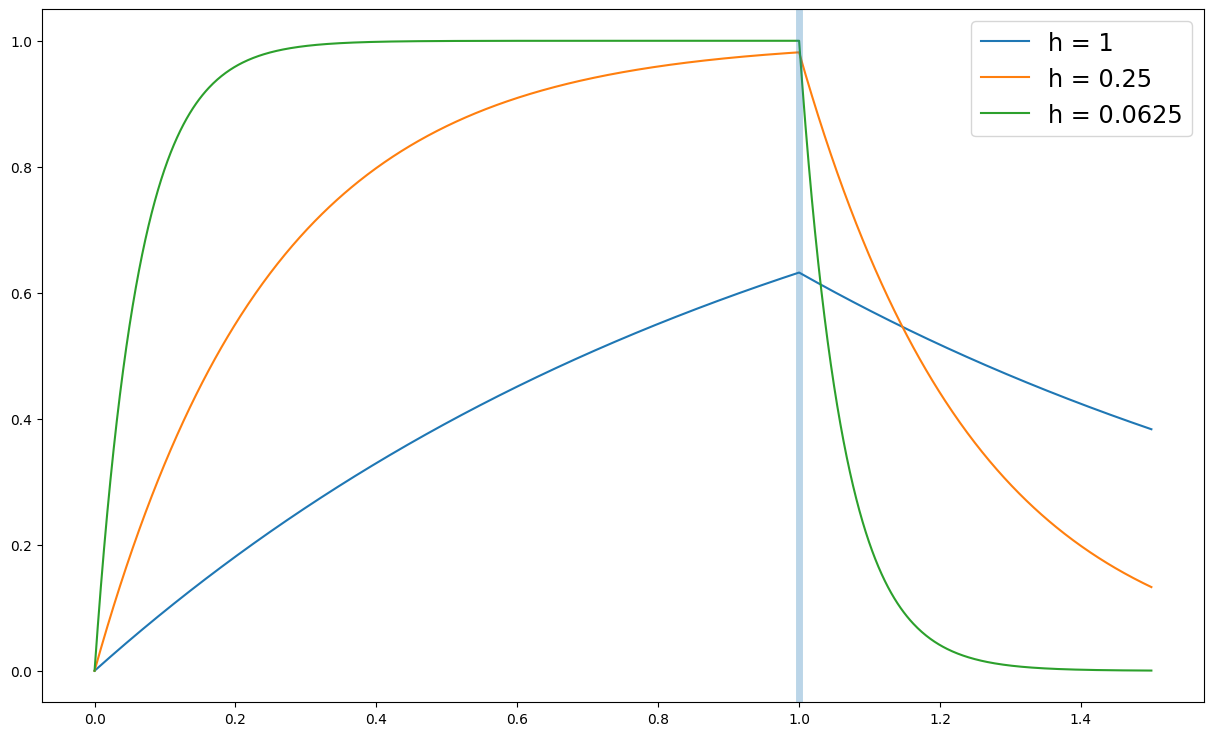
\includegraphics[width=0.7\textwidth]{img/q1_2.png}
\captionof{figure}{نمودار $\hat{p}$ به ازای مقادیر مختلف \lr{h}}
}
\subsection{}
داریم:
\begin{latin}
	$
	\bigintss \limits_{0}^a(\hat{p}(x) - p(x)) d_x
	= \bigintss_0^a \cfrac{1}{a} (e^{\cfrac{-x}{h}}) 
	= \cfrac{1}{a} [-h \  e^{\cfrac{-x}{h}}  ]_0^a
	= \cfrac{-h}{a} [ e^{\cfrac{-x}{h}}  ]_0^a
	= \cfrac{h}{a}  (1 - e^{\cfrac{-a}{h}})
	$
\end{latin}
	با جایگذاری متغیر 
	$t = \cfrac{- a}{h}$
	داریم:
	
	\begin{latin}
		$
		\cfrac{1 - e^t}{-t} \leq 0.01 \Rightarrow \cfrac{e^t - 1}{t} \leq 0.01
		$
	\end{latin}
	اگر بسط تیلور 
	$e^t = 1 + t + \cfrac{t^2}{2}$
	را بنویسیم داریم:
	\begin{latin}
		$
		1 + 0.5t \leq 0.01 \Rightarrow 0.5t \leq 0.99 \Rightarrow t \leq 1.98 \Rightarrow \cfrac{a}{h} \geq 1.98 \Rightarrow h \leq \cfrac{a}{1.98}
		$
	\end{latin}
	یعنی برای بایاس کمتر از یک درصد، 
	\lr{h}
	باید کمتر از حدودا نصف 
	\lr{a}
	باشد.
	\subsection{}
	\begin{latin}
		$
		a = 1 \Rightarrow h = \cfrac{1}{1.98} \approx 0.5
		$
	\end{latin}
	{
	\centering
	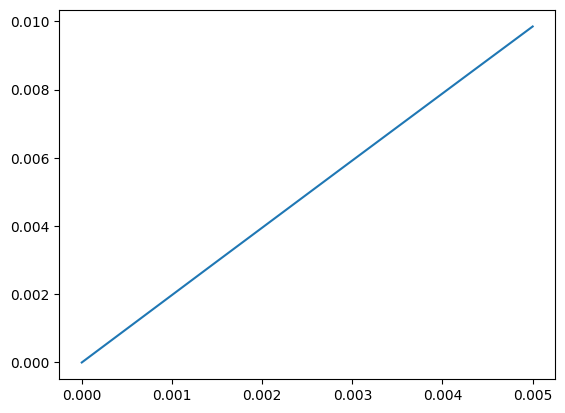
\includegraphics[width=0.7\textwidth]{img/q1_4.png}
	\captionof{figure}{مقدار $\hat{p}$ به ازای $a = 1, h = \cfrac{1}{1.98}$ در بازه $[0, 0.04]$}
	}
\newpage
\lr{\section{Shift of the Eigenvalue Spectrum}}
 \begin{latin}
 	$
 	\xi A = \lambda_A I , \xi B = \lambda_B I \Rightarrow \xi (A + B) = (\lambda_A + \lambda_B) I
 	$
 \end{latin}
 یعنی 
 $\xi$
 بردار ویژه
 $A + B$ 
 است و مقدار ویژه آن برابر با جمع دو مقدار ویژه می‌باشد.
 \subsection{}
حالت تکین وقتی پیش می‌آید که دترمینان صفر باشد یا به عبارت دیگر، یکی از مقادیر ویژه ماتریس 
$
X^TX
$
صفر باشد. واضح است که با جمع کردن ماتریس با 
$\lambda I$ 
مقدار ویژه‌های ماتریس با 
$\lambda$
جمع می‌شود 
\begin{latin}
	$
	U = x^TX \quad \xi U = \gamma I \Rightarrow \xi (U + \lambda I ) = \xi U + \xi \lambda = \gamma \xi + \lambda \xi = (\gamma + \lambda) \xi
	\Rightarrow
	\xi (U + \lambda I) = (\gamma + \lambda  )\xi
	$
\end{latin}
که یعنی با جمع 
$\lambda I$
مقادیر ویژه بردار 
\lr{U}
با 
$\lambda$
جمع می‌شوند. از آنجایی که 
$U = X^TX$ 
یک ماتریس 
\lr{semi positive definite }
است، مقادیر ویژه آن همه نامنفی هستند. پس اگر 
$\lambda$
یک مقدار مثبت باشد،‌ نتیجه یک ماتریس 
\lr{positive definite}
است که دترمینان آن مثبت است و جواب دارد.
 \subsection{}

 \begin{latin}
 	~\\
 	$
 	\text{linear} \Rightarrow 
 	\hat{\beta} = argmin (y - \beta X)^2 = (X^TX)^{-1}X^Ty 
 	\\
 	\text{Ridge} \Rightarrow 
 	\hat{\beta} = argmin(y - \beta X)^2 + ( \lambda \beta)^2 = (X^TX + \lambda I )^{-1}X^Ty 
 	$
 \end{latin}
 واضح است که در 
 \lr{ridge}
 مقدار 
 \lr{bias}
 بیشتر است زیرا بعد از فیت شدن نیز به علت وجود 
 $\lambda$ 
 مدل روی داده کامل فیت نمی‌شود. در مقابل در 
 \lr{linear regression}
 چون هدف فیت شدن کامل روی داده است بایاسی اضافه نمی‌شود و بایاس موجود ناشی از داده است. 
 
 در 
 \lr{ridge}
 چون یکی از اهداف کم بودن مقدار 
 $\beta$
 می‌باشد، احتمال بیش‌برازش کمتر است. برای مثال ممکن است مدل به دو ویژگی در مقابل هم،  امتیاز های قرینه ولی بزرگی بدهد که روی داده آموزش به طور کامل خنثی شوند ولی موقع تست چون ممکن است مقدار این ویژگی ها اندکی باهم تفاوت داشته باشد، منجر به خطای بالایی خواهد شد. ولی در 
 \lr{ridge}
 با جلوگیری از زیاد شدن 
 $\beta$
 جلوی این مورد گرفته می‌شود.
 
 برای جمع بندی، 
 \lr{ridge}
 کمی 
 \lr{bias}
 بیشتری دارد ولی 
 \lr{variance}
 کمتری دارد. این 
 \lr{tradeoff}
 را می‌توان با مقدار 
 $\lambda$
 کنترل کرد.
\newpage
\lr{\section{Optimizing a Kernel}}
\subsection{}
\begin{latin}
	$
	L(x_i ) = \sum_i  (y_i ^2 + \hat{y_i}^2 - 2 y_i \hat{y_i} ) =  (y_i  - (\cfrac{\sum_j K(x_i, x_j)y_i}{\sum_j K(x_i, x_j)})) ^ 2 
	$
\end{latin}
اگر برای 
$L(x_i)$
مقدار خود 
$x_j = x_i$
نیز درنظر گرفته شود، احتمال بیش‌برازش وجود دارد پس بهتر است که خود متغیر درنظر گرفته نشود پس داریم:
\begin{latin}
	$
	L 
	=\sum_i  (y_i ^2 + \hat{y_i}^2 - 2 y_i \hat{y_i} ) 
	=  \sum_i  (y_i  - (\cfrac{\sum_{j \neq i} K(x_i, x_j)y_i}{\sum_{j \neq i} K(x_i, x_j)})) ^ 2 
	\\
	= \sum_i  (y_i  - (\cfrac{\sum_{j \neq i} e^{-(x_i - x_j)W (x_j - xI)^T } y_i}{\sum_{j \neq i} e^{-(x_i - x_j)W (x_j - xI)^T} })) ^ 2 
	$
\end{latin}
\subsection{}
\lr{\section{KNN and the Curse of Dimensionality}}
\lr{\subsection*{a}}
اگر بازه 
$[a, b]$
انتخاب شود باید مقدار 
$P(a \leq x \leq b)$
حساب شود. در توزیع یکنواخت این عبارت برابر است با طول بازه تقسیم بر طول کل که در این حالت خاص برابر با 
$0.1$
می‌باشد.
\lr{\subsection*{b}}
باتوجه به اینکه دو ویژگی از هم مستقل هستند احتمال آن‌ها در هم ضرب می‌شود یعنی برابر است با 
$0.01$
\lr{\subsection*{c}}
مشابه قسمت قبل با ضرب احتمال‌ها داریم:
\begin{latin}
	$
	P = 0.1 ^ p = 0.1^100
	$
\end{latin}
\lr{\subsection*{d}}
اگر تعداد داده نسبت به ابعاد بصورت نمایی رشد نکند، برای تخمین هر نقطه داده کمی موجود است و نمی‌توان با دقت خوبی پیش‌بینی کرد.

در روش 
\lr{parzen}
این مشکل به این صورت رخ پیدا می‌کند که جاهای زیادی در 
\lr{pdf estimate}
صفر می‌باشد (زیرا داده‌ای یافت نشده است.)
در روش 
\lr{KNN}
این مشکل به اینصورت رخ می‌دهد که پنجره بزرگ و بزرگ تر می‌شود و احتمالا از داده‌های دور استفاده شود که نتیجتا تخمین خوبی نمی‌دهد.
\section{Choosing Metrics}
\lr{\subsection*{a}}
استفاده از 
\lr{cosine}
بهتر است زیرا در مقادیری که ذکر شد،‌نسبت کافئین به شکر (یا برعکس) جداکننده بهتری نسبت به شکر یا کافئین به تنهایی است.
\lr{\subsection*{b}}
در اینجا چون بردار صفر وارد می‌شود نسبت کافی نیست (اگر صفر هم نبود احتمال اشتباه گرفتن آب با انرژی زا وجود داشت زیرا نسبت تقریبا یکسانی دارند.) در اینجا استفاده از فاصله اقلیدسی منطقی است زیرا مقدار عددی ویژگی‌ها اهمیت دارد.
\lr{\subsection*{c}}
چون مقدار ها عددی نیستند فاصله همینگ بهتر است.
\lr{\subsection*{d}}
گزینه ۳. در درخت تصمیم، میزان تاثیر ویژگی‌ها سنجیده می‌شود ولی در سنجش فاصله این عدد سنجیده نمی‌شود. 

\lr{\section{Kernel Ridge Regression}}
\lr{\subsection*{a}}
با استفاده از 
\lr{vector notation}
داریم:
\begin{latin}
	$
	J = \cfrac{1}{2}  \sum (X \theta - Y )^2 + \cfrac{\lambda}{2} |\theta|^2
	= \cfrac{1}{2} (X \theta - Y )^T(X \theta - Y ) + \cfrac{\lambda}{2} \theta^T \theta
	\\\\
	= \cfrac{1}{2} (\theta ^ T X^T X \theta - \theta ^ T X^T Y - Y^T X \theta + Y^T Y + \lambda \theta^T \theta )
	$
\end{latin}
این عبارات عدد هستند پس ترانهاد آن‌ها باهم برابر است. دوعبارت وسط ترانهاد همدیگر هستند و باهم برابر هستند پس داریم:
\begin{latin}
	$
	J = \cfrac{1}{2} (\theta ^ T X^T X \theta^T - 2 \theta^T X^T Y + Y^T Y + \lambda \theta^T \theta)
	$
\end{latin}
با مشتق گرفتن نسبت به $\theta$ و صفر گذاشتن داریم:
\begin{latin}
	$
  \cfrac{1}{2}  (2X^T X \theta - 2 X ^ T Y  + 2 \lambda \theta) = 0 
  \Rightarrow
  (X^T X + \lambda I ) \theta =  X ^ T Y  
  \\
  \Rightarrow
  \theta = ((X^T X + \lambda I ) ^{-1}  X^T Y)
	$
\end{latin}
\lr{\subsection*{b}}
حل نشده است.

\lr{\section{Deriving Linear Regression}}
\lr{\subsection*{a}}
داریم:
\begin{latin}
	$
	E(yx) = w^T x^2 + \epsilon x = w^T E(x^2) + E(\epsilon) E(x) = w^T \Sigma_x
	$
\end{latin}
\lr{\subsection*{b}}
می‌دانیم بهترین تخمینگر میانگین جامعه، میانگین نمونه است. پس داریم:
\begin{latin}
	$
	E(yx | D) = \cfrac{1}{n} \sum\limits_{i = 1}^n (x_i y_i)
	$
\end{latin}
\lr{\subsection*{c}}
داریم:
\begin{latin}
	$
	L = E((w^T x  - y)^2) \xrightarrow{minimize\ loss \rightarrow derviative\ from\ w} E(2(w^Tx - y)x) = 0 \Rightarrow E(w^Tx^2) = E(yx)
	\Rightarrow w^T \Sigma_x \Rightarrow \hat{w} = (\cfrac{E(yx)}{\Sigma_X})^T = (\cfrac{\Sigma_{xy}}{\Sigma_x})^T
	$
\end{latin}
\lr{\subsection*{d}}
روی صورت اتفاقی نمی‌افتد زیرا مقدار آن از روی نمونه حساب شد. ولی در مخرج، درواقع 
$
E(X^2)
$
بود. پس یعنی باید با مربع میانگین جمع شود پس داریم:
\begin{latin}
	$
	\hat{w} = \cfrac{\Sigma_{xy}}{\Sigma_x + \mu_x^2}
	$
\end{latin}


\lr{\subsection*{e}}
بله. درجایی از محاسبات از نرمال بودن استفاده نشد. صرفا اگر نرمال باشد می‌توان چیزهایی مثل بازه اطمینان و غیره را حساب کرد.
	
	\lr{\section{A Bayesian Interpretation of Lasso}}
	\lr{\subsection*{a}}
	داریم:
	\begin{latin}
		$
		f(w | (y | x)) = \cfrac{f(y | x, w) f(w)}{f(y | x)}
		$
	\end{latin}
	چون مقدار 
	\lr{w}
	در مخرج نقشی ندارد و برای همه 
	\lr{w}
	ها یکسان است می‌توان از آن صرفنظر کرد. پس یعنی باید 
	\lr{w}
	ای پیدا کرد که مقدار 
	$f(w)f(y | x, w)$
	در آن بیشینه باشد. پس داریم:
	\begin{latin}
		$
		f(w | (y|x)) \propto f(w)f(y | x, w) = \cfrac{1}{2b} e^{\cfrac{-|w|}{b}} * \prod \cfrac{1}{\sigma \sqrt{2\pi}} e^{-\cfrac{(y - w.x)^2}{2\sigma^2}}
		$
	\end{latin}
	با حذف مقادیری که 
	\lr{w}
	در آن‌ها نقشی ندارد داریم:
	\begin{latin}
		$
		f(w | (y | x)) \propto e^{-(\cfrac{|w|}{b} + \sum  \cfrac{(y - w.x)^2}{2\sigma^2})}
		$
	\end{latin}
		\lr{\subsection*{b}}
		با گرفتن لگاریتم از حاصل قسمت قبل داریم :
		\begin{latin}
			$
			l = -(\cfrac{|w|}{b} + \sum  \cfrac{(y - w.x)^2}{2\sigma^2})
			$
		\end{latin}
		از آنجایی که لگاریتم صعودی است کافیست مقدار 
		\lr{l}
		بیشینه شود تا 
		\lr{maximum likelihood}
		بدست آید. همچنین می‌توان یک عدد ثابت را ضرب کرد پس داریم:
		\begin{latin}
			$
		\hat{w} = argmax \cfrac{1}{2b\sigma^2} |w| + \sum (y - w.x)^2
			$
		\end{latin}
		که این همان چیزی است که در سوال آمده و مقدار 
		$\lambda$
		برابر است با:
		\begin{latin}
			$
			\cfrac{1}{2b\sigma^2}
			$
		\end{latin}
	\lr{\section{Parzen Window Classification with Gaussian Kernel}}
	موارد در نوتبوک 
	\lr{10.ipynb}
	حل شده‌اند. در هر دو مورد کلاس ۱ انتخاب شد. 
	\begin{table}[h!]
		\centering
		
		\caption{احتمال تخمین زده شده برای هر نقطه با $h = 1$}
		\begin{latin}
			\label{tab:class-probabilities}
			\begin{tabular}{ccccc}
				\textbf{Coordinates} & $\mathbf{P(\omega_1)}$ & $\mathbf{P(\omega_2)}$ & $\mathbf{P(\omega_3)}$   \\
				$(0.5, 1.0, 0.0)$ 1 & 0.1259 & 0.4711 & 0.3775 \\
				$(0.31, 1.51, -0.5)$  & 0.1534 & 0.4828 & 0.2050  \\
				$(-0.3, 0.44, -0.1)$   & 0.1399 & 0.3783 & 0.1771  \\
			\end{tabular}
		\end{latin}
	\end{table}
	
	
	\begin{table}[h!]
		\centering
		\caption{احتمال تخمین زده شده برای هر نقطه با $h = 0.1$}
		\begin{latin}
		\begin{tabular}{cccc}
			\textbf{Coordinates} & $\mathbf{P(\omega_1)}$ & $\mathbf{P(\omega_2)}$ & $\mathbf{P(\omega_3)}$ \\
			$(0.5, 1.0, 0.0)$ & $8.77 \times 10^{-20}$ & $6.77 \times 10^{-5}$ & $8.00 \times 10^{-17}$ \\
			$(0.31, 1.51, -0.5)$ & $2.87 \times 10^{-20}$ & $1.20 \times 10^{-5}$ & $2.16 \times 10^{-25}$ \\
			$(-0.3, 0.44, -0.1)$ & $3.64 \times 10^{-12}$ & $3.78 \times 10^{-4}$ & $1.06 \times 10^{-39}$ \\
		\end{tabular}
				\end{latin}
	\end{table}
	{
	\centering
	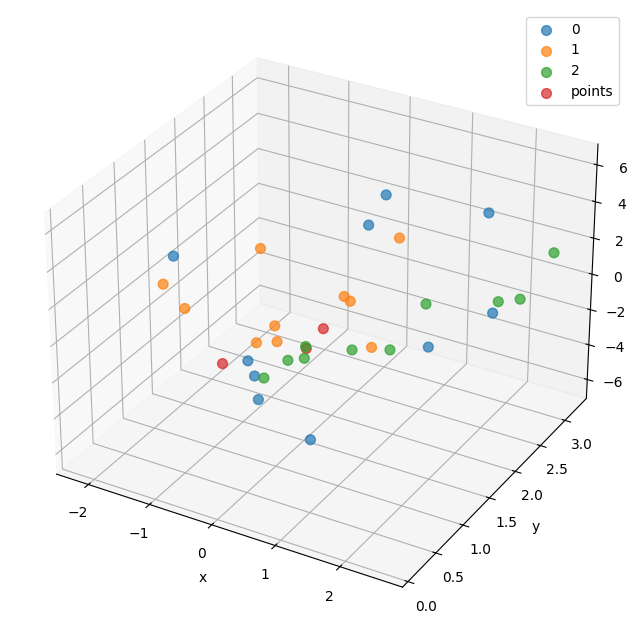
\includegraphics[width=0.5\textwidth]{img/q10.png}
	\captionof{figure}{نمودار پراکندگی نقاط}
	}
	
	\lr{\section{Maximum likelihood estimation}}
	\lr{\subsection*{a,b}}
	\begin{latin}
		$
		f(x | \mu, \sigma) \propto \cfrac{1}{\sigma}\  e^{-\cfrac{(x - \mu)^2}{2\sigma^2}}
		$
	\end{latin}
	برای تخمین 
	\lr{mle}
	باید این عبارت را براساس 
	$\mu$
	و 
	$\sigma$
	بیشینه کرد. برای میانگین واضح است که کمترین مقدار داخل پرانتز (و درنتیجه بیشترین مقدار توان) وقتی است که مقدار 
	$\sum (x - \mu)^2$
	کمینه باشد.با باز کردن این عبارت داریم:
	\begin{latin}
		$
		\mu = argmin \sum x^2 + \mu^2 -2x\mu = argmin( n\mu^2 - 2n\bar{x}\mu )= \mu^2 - 2\mu \bar{x} \Rightarrow \mu = \bar{x}
		$
	\end{latin}
	برای واریانس داریم:
\begin{latin}
	$
	l = \sum (-ln(\sigma) - \cfrac{(x - \mu)^2}{2\sigma^2})
	$
\end{latin}
با مشتق گیری برحسب 
$\sigma$
داریم:
\begin{latin}
	$
	-(\cfrac{n}{\sigma} + \sum  \cfrac{(x - \mu)^2}{2} (\cfrac{-2}{\sigma^3}) ) 
	= \cfrac{-1}{\sigma} (n - \sum \cfrac{(x - \mu)^2}{\sigma^2} ) = 0 \Rightarrow \sigma^2 =\sum \cfrac{(x - \mu)^2}{n}
	$
\end{latin} 
که با محاسبه با اعداد بدست می‌آید:
\begin{latin}
	$
	\mu_{theory} = 100.48049999999999 \qquad
	\sigma_{theory} = 14.707769026946268
	$
\end{latin}
مقدار عددی نیز چیزی در همین حدود شد:
\begin{latin}
	$
	\mu_{numeric} = 100.48050398080368 \qquad
	\sigma_{numeric} = 14.707763577982128
	$
\end{latin}
{
	\centering
	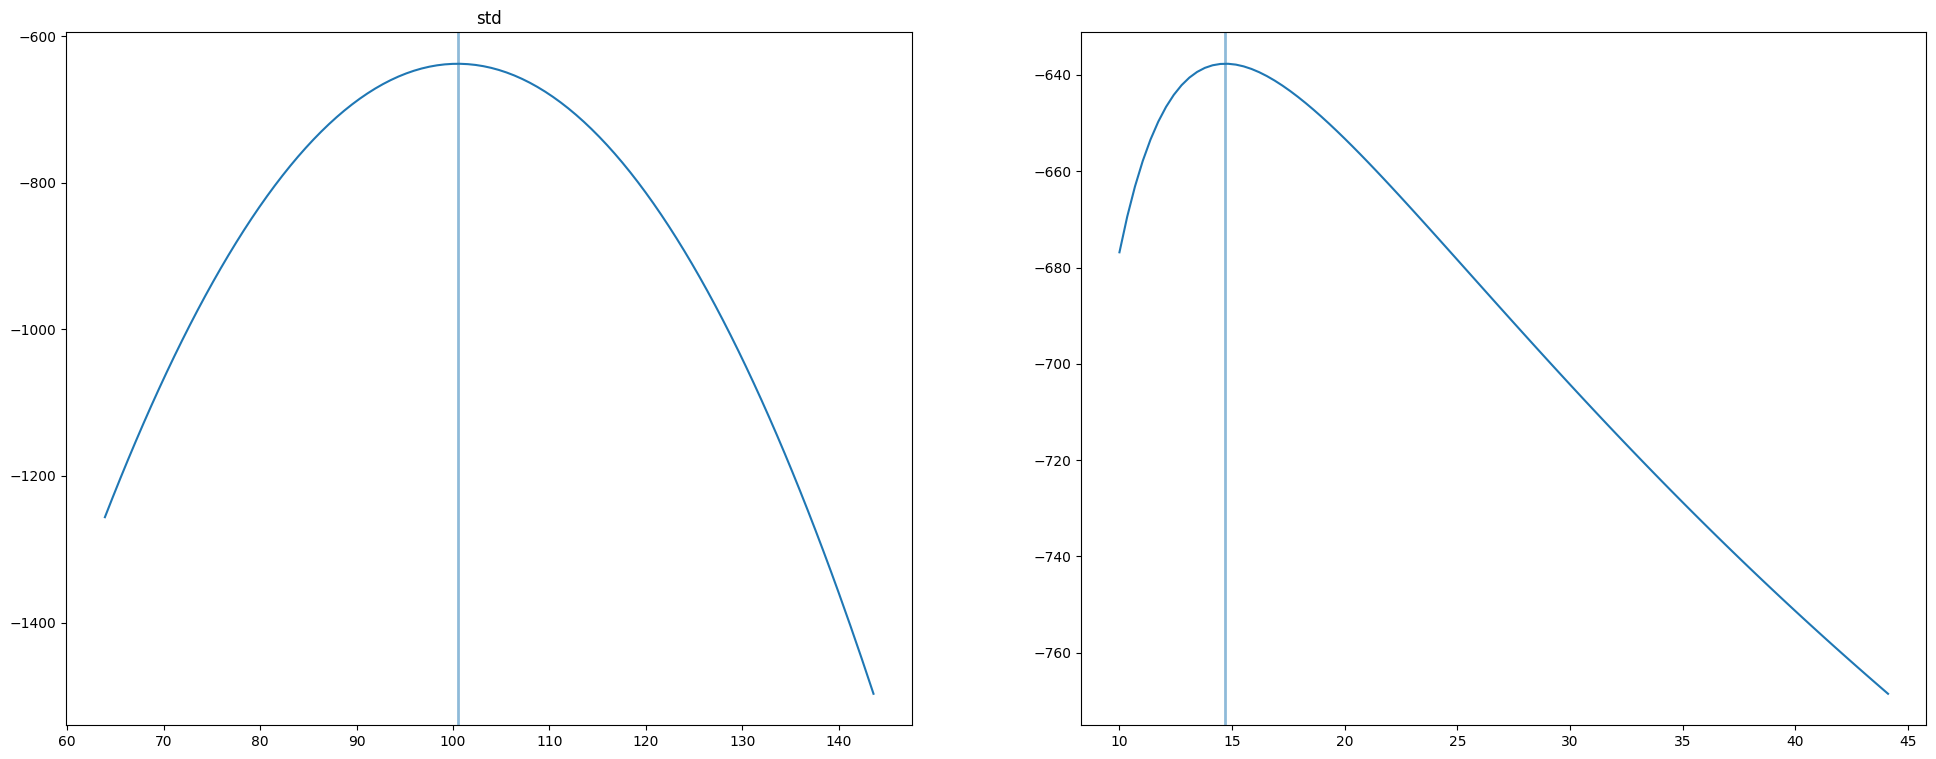
\includegraphics[width=0.8\textwidth]{img/q11_1.png}
	\captionof{figure}{میزان \lr{likelihood} به ازای مقادیر مختلف میانگین و واریانس. مقادیر محاسبه شده به صورت تئوری به صورت خط به نمایش در آمده‌اند.}
}
\lr{\subsection*{c,d}}
سوال درواقع 
\lr{fisher information}
را می‌خواهد:
\begin{latin}
	$
	I^{-1}= \begin{bmatrix}
		\cfrac{\sigma^2}{n} & 0 \\
		0 & \cfrac{2\sigma^4}{n}
	\end{bmatrix}
	\approx 
	\begin{bmatrix}
		1.081 & 0 \\
		0 & 467.93
	\end{bmatrix}
	$
	
\end{latin}
هم در حالت عددی و هم در حالت تئوری این‌مقدار تقریبا برابر است.
\lr{\subsection*{e}}
\begin{latin}
	$
	\cfrac{(n - 1) s^2}{\sigma^2} \sim \chi_{n - 1}^2
	$
\end{latin}
با استفاده از این فرمول بازه با استفاده از کد در نوتبوک محاسبه شد. بازه اطمینان 
\lr{95}
درصد انحراف معیار برابر است با:
\begin{latin}
	$
	[13.4274, 16.3507]
	$
\end{latin}
\lr{\subsection*{f}}
\begin{itemize}
	\item 
	برای \lr{Z test} چون سایز نمونه از 
	\lr{30}
	بزرگ تر است می‌توان از خود \lr{Z}استفاده کرد. چون راجع به \lr{Alternative Hypotheis} حرفی زده نشده، تست 
	\lr{two sided}
	درنظر گرفته می‌شود.
	طبق فرمول داریم:
	\begin{latin}
		$
		z = \cfrac{100.48 - 103}{\cfrac{14.7}{\sqrt{200}}} \approx -2.42
		\Rightarrow p\_value = 2*(1 - Z_{-2.42}) \approx 0.01
		$
	\end{latin}
	پس یعنی فرض صفر رد می‌شود. 
\end{itemize}
%	\begin{latin}
%	\printbibliography[heading=none]
%\end{latin}

\end{document}